\chapter{Results}


The evaluation results were obtained using standard and commonly used MIR tools, frameworks, and metrics. These include the MSAF \cite{MSAF} implementation for segmentation algorithms, the SALAMI dataset \cite{Smith2011DESIGNANNOTATIONS} for evaluation ground truth, and $mireval$ Python package \cite{RaffelMir_eval:METRICS} for metric computation.

Table \ref{ta:results} provides a comparative analysis across four different features using three different segmentation algorithms. The results reveal that the performance of the algorithms varies depending on the type of feature. For instance, the CQT feature exhibits the highest precision (0.570), recall (0.339), and f-measure (0.353) when processed with the Foote algorithm. This table also proves that it is possible to achieve competitive perfor-
mance to traditional handcrafted signal processing methods by learning only from unlabeled audio files.

The visual representation of these results is also provided in Figure \ref{fig:boxplotmetrics} to better understand the distribution of the metrics for each feature.

Table \ref{tab:comparison_table} and Figure \ref{fig:enter-label} offer a comparison of the current study's boundary detection F-measure results with those of previous studies using unsupervised methods. The most accurate result was reported in 2019 by McCallum \cite{deepfeaturesegment} who used a CNN on CQT and achieved an F-measure of 0.535. The current study's approach using raw waveforms as input and CNN as the method yielded an F-measure of 0.288.

%%%%%%%%%%%%%%%%%%%%%%%%%%%%

\begin{table}[ht]
\centering
\small
\begin{tabularx}{\textwidth}{>{\centering\arraybackslash}p{4.5cm}>{\centering\arraybackslash}X>{\centering\arraybackslash}X>{\centering\arraybackslash}X}
\toprule
\textbf{Training dataset [Ref]}  & \textbf{Precision} & \textbf{Recall} & \textbf{F-measure} \\
\midrule
\addlinespace
GTZAN \cite{GTZAN} & 0.228 & 0.171 & 0.185 \\
\addlinespace
MSD \cite{MSD} &  \textbf{0.333} &  \textbf{0.280} & \textbf{0.288} \\
\addlinespace
\bottomrule
\end{tabularx}
\caption[GTZAN-trained versus MSD-trained embeddiograms]{\small{Comparison of precision, recall, and F-measure for GTZAN-trained versus MSD-trained embeddiograms on SALAMI dataset computed using the Structural Feature (SF)\cite{sf} algorithm.}}
\label{tab:comparison_table}
\end{table}

%%%%%%%%%%%%%%%%%%%%%%%%%%%%

Table \ref{tab:comparison_table} compares the performance of the Structural Feature (SF) algorithm on the SALAMI dataset, utilizing two distinct sets of embeddiograms as input features. These embeddiograms were respectively generated with the neural network trained using the GTZAN and MSD datasets.

The results show a clear advantage for the SF algorithm when it is trained on the MSD dataset, as compared to the GTZAN dataset. Specifically, the precision, recall, and f-measure are all higher for the MSD-trained algorithm.

The precision, recall, and f-measure metrics in Table \ref{tab:comparison_table} evaluate the performance of the Structural Feature (SF) algorithm using GTZAN and MSD-trained embeddiograms. Precision indicates the proportion of correctly predicted boundaries. The MSD-trained algorithm outperforms the GTZAN-trained one, scoring 0.333 versus 0.228. Recall measures the algorithm's success in detecting all actual boundaries; again, the MSD-trained version shows better performance with a score of 0.280 against GTZAN's 0.171. F-measure, a metric that balances precision and recall, also favors the MSD-trained algorithm, with a score of 0.288 compared to 0.185 for the GTZAN-trained version.

%%%%%%%%%%%%%%%%%%%%%%%%%%%%

\newsavebox\embeddiobSF
\begin{lrbox}{\embeddiobSF}
   $\begin{aligned}
     \textbf{0.333} & \quad 0.280 & \quad 0.288
    \end{aligned} $
\end{lrbox}

\newsavebox\embeddiobFoote
\begin{lrbox}{\embeddiobFoote}
   $\begin{aligned}
     0.275 & \quad 0.318 & \quad 0.280
    \end{aligned} $
\end{lrbox}

\newsavebox\embeddiobCNMF
\begin{lrbox}{\embeddiobCNMF}
   $\begin{aligned}
     0.248 & \quad 0.296 & \quad 0.254
    \end{aligned} $
\end{lrbox}

\newsavebox\pcpSF
\begin{lrbox}{\pcpSF}
   $\begin{aligned}
     0.311 & \quad 0.324 & \quad 0.305
    \end{aligned} $
\end{lrbox}

\newsavebox\pcpFoote
\begin{lrbox}{\pcpFoote}
   $\begin{aligned}
     0.288 & \quad \textbf{0.331} & \quad 0.295
    \end{aligned} $
\end{lrbox}

\newsavebox\pcpCNMF
\begin{lrbox}{\pcpCNMF}
   $\begin{aligned}
     0.228 & \quad 0.310 & \quad 0.250
    \end{aligned} $
\end{lrbox}

\newsavebox\tonnetzSF
\begin{lrbox}{\tonnetzSF}
   $\begin{aligned}
     0.312 & \quad 0.312 & \quad 0.300
    \end{aligned} $
\end{lrbox}

\newsavebox\tonnetzFoote
\begin{lrbox}{\tonnetzFoote}
   $\begin{aligned}
     0.272 & \quad 0.317 & \quad 0.280
    \end{aligned} $
\end{lrbox}

\newsavebox\tonnetzCNMF
\begin{lrbox}{\tonnetzCNMF}
   $\begin{aligned}
     0.212 & \quad 0.306 & \quad 0.237
    \end{aligned} $
\end{lrbox}

\newsavebox\cqtSF
\begin{lrbox}{\cqtSF}
   $\begin{aligned}
     0.311 & \quad \textbf{0.339} & \quad \textbf{0.312}
    \end{aligned} $
\end{lrbox}

\newsavebox\cqtFoote
\begin{lrbox}{\cqtFoote}
   $\begin{aligned}
     \textbf{0.570} & \quad 0.311 & \quad \textbf{0.353}
    \end{aligned} $
\end{lrbox}

\newsavebox\cqtCNMF
\begin{lrbox}{\cqtCNMF}
   $\begin{aligned}
     \textbf{0.296} & \quad \textbf{0.311} & \quad \textbf{0.287}
    \end{aligned} $
\end{lrbox}

%%%%%

\begin{table}
  \centering
  \begin{adjustbox}{width=\textwidth}
  \begin{threeparttable}
    \begin{tabular}{c|c|c|c|c} 
\toprule
     \textbf{Feature} & \textbf{SF} & \textbf{Foote} & \textbf{CNMF} 
     \\ \midrule 
     PCP & \usebox{\pcpSF} & \usebox{\pcpFoote} & \usebox{\pcpCNMF} \\\hline
     Tonnetz & \usebox{\tonnetzSF} & \usebox{\tonnetzFoote} & \usebox{\tonnetzCNMF} \\\hline
     CQT & \usebox{\cqtSF} & \usebox{\cqtFoote} & \usebox{\cqtCNMF} \\\hline
     Embeddiogram & \usebox{\embeddiobSF} & \usebox{\embeddiobFoote} & \usebox{\embeddiobCNMF} \\
     \bottomrule
    \end{tabular}
    \caption[Metric comparison: audio features and segmentation algorithms]{Comparison of precision (left column), recall (middle column), and f-measure (right column) metrics for different features using the Structural Feature (SF)\cite{sf}, Checkerboard-like Kernel (Foote) \cite{Foote2000AutomaticNovelty}, and Convex Non-negative Matrix Factorization (CNMF) \cite{NietoCONVEXIDENTIFICATION} algorithms on the SALAMI dataset. The sliding windowed segments across the input signal is 4 seconds long.}\label{ta:results}
  \end{threeparttable}
  \end{adjustbox}
\end{table}

%%%%%%%%%%%%%%%%%%%%%%%%%%%

\begin{figure}
    \centering
    \includegraphics[width=\textwidth]{figures/images/boxplot.png}
    \caption[Metric comparison for different audio features.]{\small{Boxplot visual comparison of different features' average precision, recall, and f-measure. Sliding windowed segments across the audio signal input signal is 4 seconds.}}
    \label{fig:boxplotmetrics}
\end{figure}

%%%%%%%%%%%%%%%%%%%%%%%%%%%%

\begin{table}[ht]
\begin{threeparttable}
\centering
\small
\begin{tabularx}{\textwidth}{
  >{\centering\arraybackslash}p{4.5cm}
  >{\centering\arraybackslash}X
  >{\centering\arraybackslash}X
  >{\centering\arraybackslash}X}
\toprule
\thead{\textbf{Authors [Ref], Year}} & \thead{\textbf{Input}\tnote{1}} & \thead{\textbf{Method}} & \thead{\textbf{F-measure}} \\
\midrule
Turnbull et al. \cite{Turnbull2007ABOOSTING}, 2007 & MFCCs, chromas, spectrogram & Boosted Decision Stump  & 0.378 \\
\addlinespace
Kaiser et al. \cite{27}, 2012 & SSM & Novelty measure  & 0.286 \\
\addlinespace
Sargent et al. \cite{34}, 2011 & MFCCs, chromas & Viterbi  & 0.356 \\
\addlinespace
McFee \& Ellis \cite{20}, 2013 & MLS & Fisher’s Linear Discriminant  & 0.317 \\
\addlinespace
Nieto \& Bello \cite{28}, 2014 & MFCCs, chromas & Checkerboard-like kernel  & 0.299 \\
\addlinespace
Cannam et al. \cite{29}, 2015 & Timbre-type histograms & HMM  & 0.213 \\
\addlinespace
Nieto \cite{30}, 2016 & CQT Spectrogram & Linear Discriminant Analysis  & 0.299 \\
\addlinespace
Cannam et al. \cite{29}, 2017 & Timbre-type histograms & HMM  & 0.212 \\
\addlinespace
Ullrich et. al \cite{22}, 2014 & MLS & CNN  & 0.465 \\
\addlinespace
Grill \& Schlüter \cite{4}, 2015 & MLS, SSLMs & CNN  & 0.523 \\
\addlinespace
Grill \& Schlüter \cite{Grill2015MusicAnnotations}, 2015 & MLS, PCPs, SSLMs & CNN  & 0.508 \\
\addlinespace
Hadria \& Peeterss \cite{35}, 2017 & MLS, SSLMs & CNN  & 0.291 \\
\addlinespace
McCallum \cite{deepfeaturesegment}, 2019 & CQT & CNN  & \textbf{0.535} \\
\addlinespace
Ours, 2023 & Raw waveforms & CNN  & 0.288 \\
\bottomrule
\end{tabularx}
\caption[Baseline. State-of-the-art table.]{Previous studies' boundary detection f-measure results using unsupervised methods for a 0.5s time-window tolerance. Only the top-performing algorithm for each year on the SALAMI dataset is displayed. This table has been extended from \cite{Hernandez-Olivan2021MusicFeatures}.}
\label{tab:comparison_table}
\begin{tablenotes}\footnotesize
\item[1] \textbf{Legend:} SSM: Self-Similarity Matrix, MLS: Mel Spectrogram, MFCC: Mel-Frequency Cepstral Coefficient, CQT: Constant Q-Transform, PCP: Pitch Class Profile, SSLM: Self-Similarity Lag Matrix.
\end{tablenotes}
\end{threeparttable}
\end{table}

%%%%%%%%%%%%%%%%%%%%

\begin{figure}
    \centering
    \includegraphics[width=\textwidth]{figures/images/fmeasuregraphs.png}
    \caption[Baseline. State-of-the-art graph.]{Previous studies' boundary detection f-measure results using unsupervised methods for a 0.5s time-window tolerance. Only the top-performing algorithm for each year on the SALAMI dataset is displayed. This figure has been extended from \cite{Hernandez-Olivan2021MusicFeatures}.}
    \label{fig:enter-label}
\end{figure}

The GitHub repository containing all the code needed to run the experiments can be found \href{https://github.com/oriolcolomefont/Master-Thesis.git}{HERE}.




\begin{figure}
    \centering
    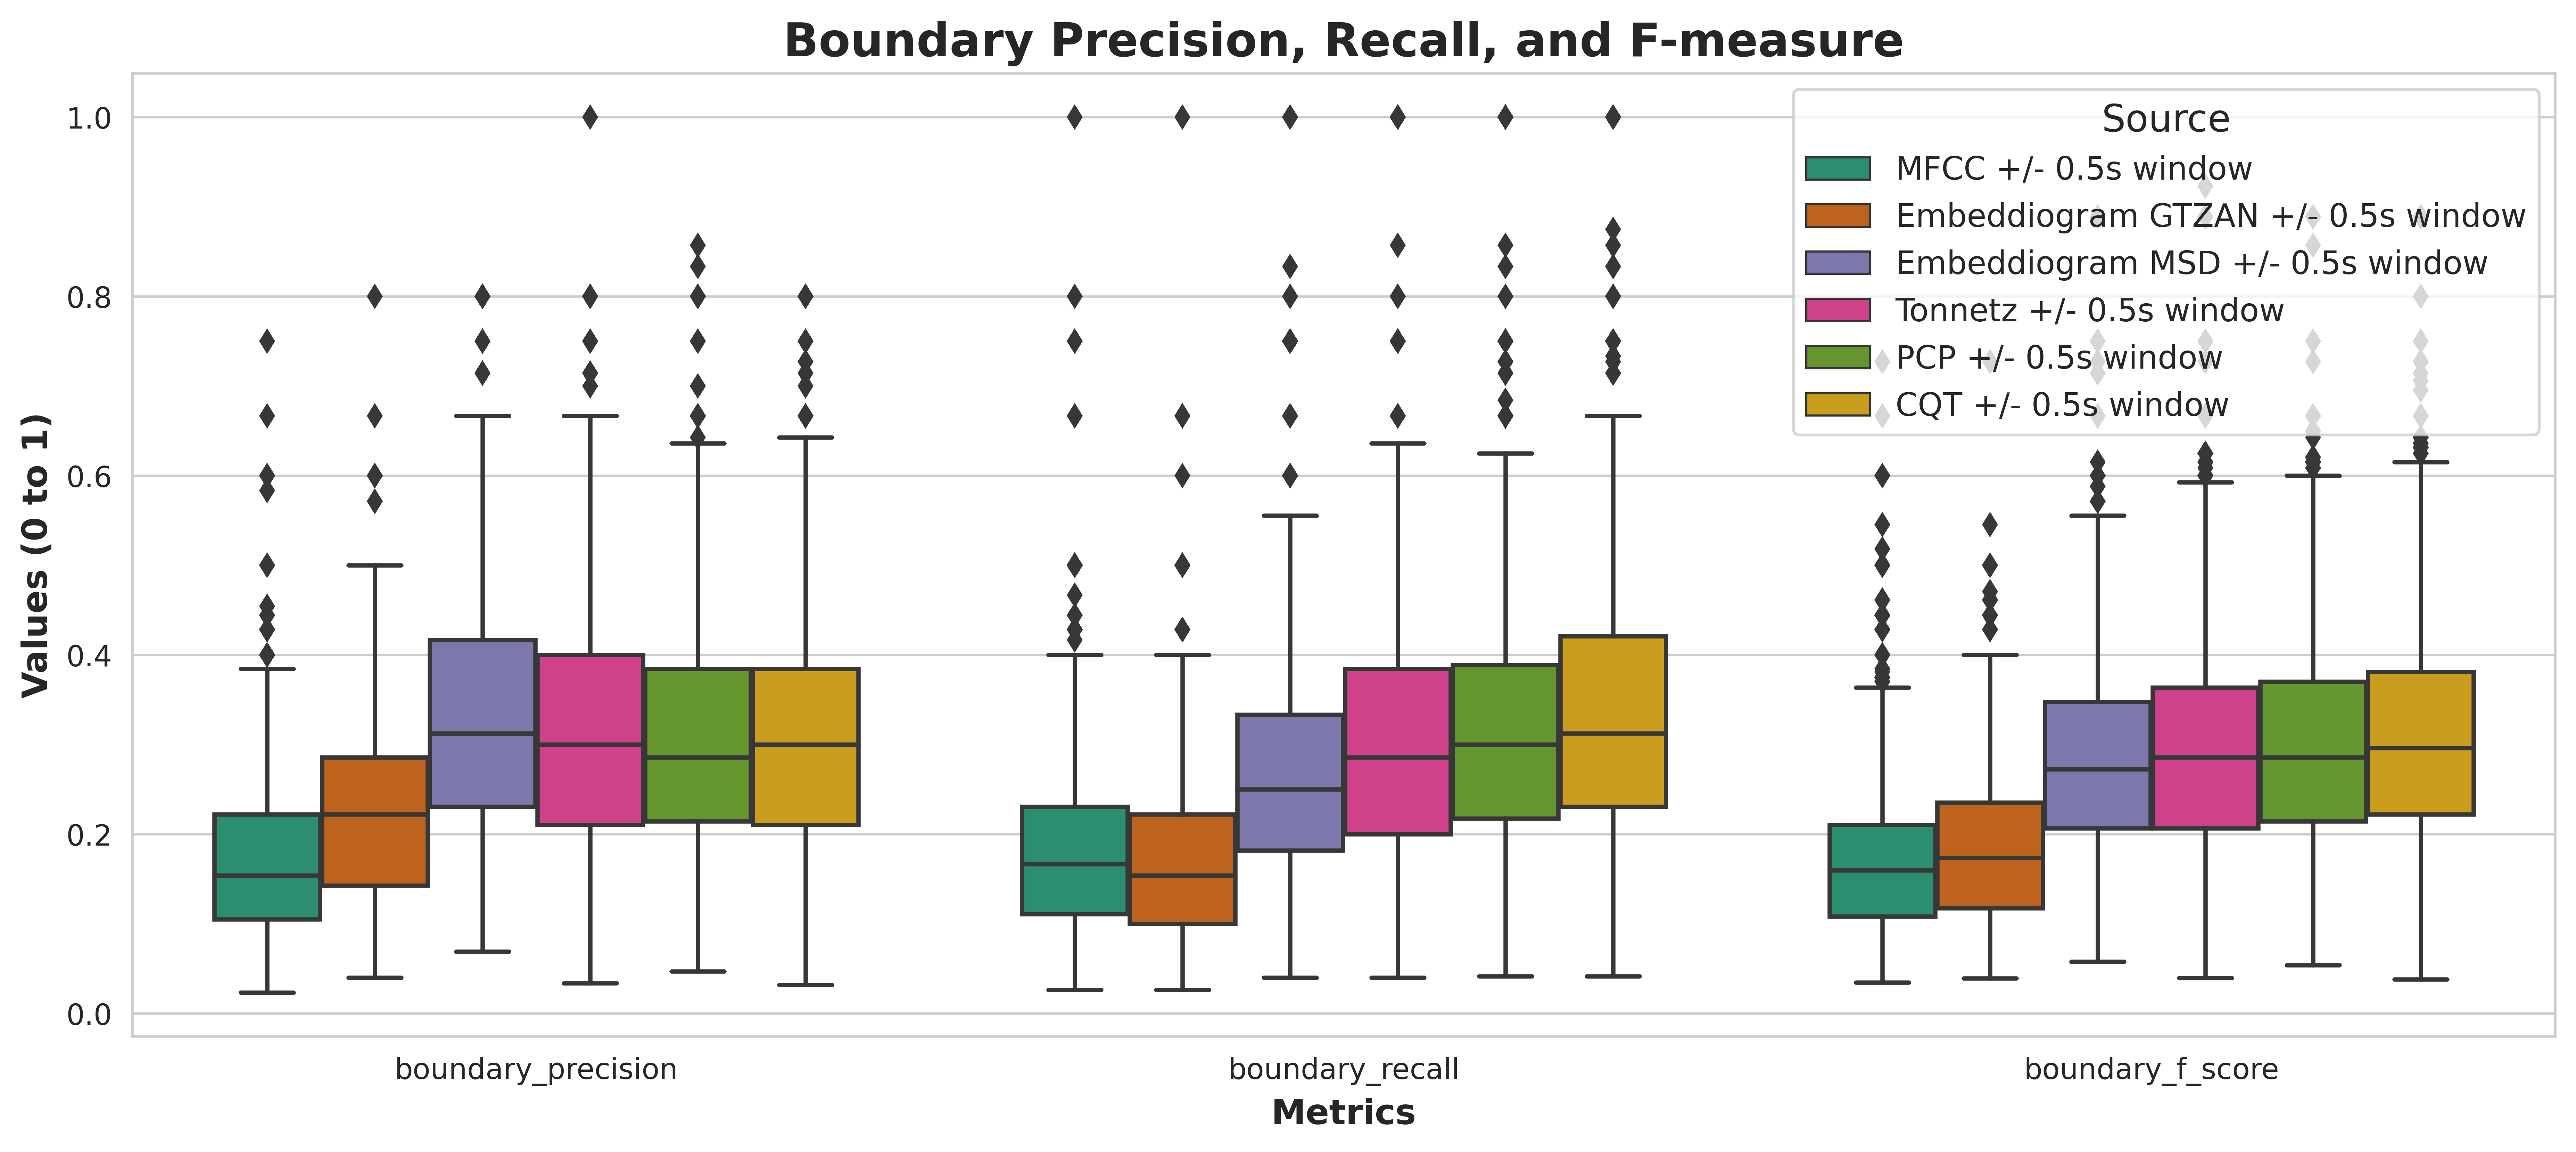
\includegraphics[width=\textwidth]{figures/images/metrics.png}
    \caption[Metric comparison for different audio features. Boxplot]{Boxplot visual comparison of precision, recall, and f-measure for different features obtained using the SF algorithm \cite{sf} on the SALAMI dataset. Sliding windowed segments across the audio signal input signal is 4 seconds}
    \label{fig:boxplotmetrics}
\end{figure}

\begin{figure}
    \centering
    \includegraphics[width=\textwidth]{figures/images/boudaryfscore.png}
    \caption[F-measure comparison for different audio features. Boxplot]{Boxplot visual comparison of f-measure for different features obtained using the SF algorithm \cite{sf} on the SALAMI dataset. Sliding windowed segments across the audio signal input signal is 4 seconds}
    \label{fig:boxplotfmeasure}
\end{figure}

\newpage


